\documentclass[twocolumn,showpacs,preprintnumbers,nofootinbib,prd,
superscriptaddress,10pt]{revtex4-2}

	%to make sure that pdflatex is used
\pdfoutput=1

\usepackage{amsmath,amssymb}
\usepackage{amsfonts}
\usepackage{mathtools}
\usepackage[normalem]{ulem}
\usepackage{textcomp}
\usepackage{enumitem}
\usepackage{bm}
\usepackage{bbm}
\usepackage{afterpage}
\usepackage{graphicx}
\graphicspath{{img/}} %setting img path
\usepackage{tensor}

\usepackage{tabularx}
\usepackage{longtable}
\usepackage{makecell}
\usepackage{multirow}
\usepackage{booktabs}


\usepackage{layouts}
\usepackage[usenames,dvipsnames]{xcolor}
\usepackage[utf8]{inputenc}
\usepackage{rotating}
\usepackage[bookmarks]{hyperref}
%\usepackage{ragged2e}
\usepackage{blindtext}
\usepackage{graphicx}
\usepackage{siunitx}
	\sisetup{output-decimal-marker={.}}
	
\usepackage{arydshln}

	%some math symbols
\newcommand{\R}{\mathbb{R}}
\newcommand{\N}{\mathbb{N}}
\DeclareMathOperator{\sign}{sign}
\renewcommand{\d}[1]{\ensuremath{\operatorname{d}\!{#1}}}
\newcommand{\dvol}[2]{\ensuremath{\operatorname{d}^{#2}\!{#1}}}
%argmin and argmax
\DeclareMathOperator*{\argmax}{arg\,max}
\DeclareMathOperator*{\argmin}{arg\,min}

\newcommand{\scalar}[2]{\langle #1|#2 \rangle}
\newcommand{\scalarnonorm}[2]{\langle #1|#2 \rangle_{\text{not normalized}}}
\newcommand{\rescalar}[2]{( #1 |#2 )}
\newcommand{\rescalarwide}[2]{\left( #1 \lvert #2 \right)}
\newcommand{\imscalar}[2]{[ #1|#2 ]}


% comments command
\newcommand{\stefano}[1]{{\textcolor{blue}{\texttt{SS: #1}} }}
\newcommand{\sarah}[1]{{\textcolor{red}{\texttt{SC: #1}} }}
\newcommand{\bhooshan}[1]{{\textcolor{cyan}{\texttt{BG: #1}} }}


\begin{document}

	%%%%%%%%%%%%%%%%%%%%%%%%%%%%%%%%% ABSTRACT
\begin{abstract}
	We introduce a novel method to generate a bank of gravitational-waveform templates of binary Black Hole (BBH) coalescences for matched-filter searches in LIGO, Virgo and Kagra data. Unlike the standard approach, our method relies on a numerical metric approximation of the distance between templates, which makes the template placement orders-of-magnitude faster than with existing techniques.
	Our method applies to a variety of different manifolds of signals and is particularly suitable for covering high-dimensional spaces, such as those associated with precessing and/or eccentric waveforms.
	We compare our method with the state-of-the-art stochastic placement code and find that our code slightly overcovers the space, while achieving similar efficiency in recovering signals. To demonstrate the capabilities of our code, we generate a bank for precessing Black Holes, a bank for intermediate-mass Black Holes with higher-order modes, and an eccentric bank, and show that they cover the space in a satisfactory way.
	Our publicly released code \texttt{mbank} will enable searches of high-dimensional regions of BBH signal space, hitherto unfeasible due to the prohibitive cost of bank generation.
\end{abstract}
	
	%%%%%%%%%%%%%%%%%%%%%%%%%%%%%%%%% TITLE
 %\title{Metric template placement for high dimensional regions of compact binary mergers}
 %\title{Fast metric-based template placement for gravitational-waves from novel compact binary mergers}
 %\title{Mbank: fast metric-based template banks for gravitational wave searches for exotic compact binaries}
 %\title{Template banks for exotic compact binaries}
 %\title{Template banks for novel compact binaries}
 \title{Gravitational-wave template banks for novel compact binaries}
	\author{Stefano \surname{Schmidt}}
		\email{s.schmidt@uu.nl}
        \affiliation{Nikhef, Science Park 105, 1098 XG, Amsterdam, The Netherlands}
        \affiliation{Institute for Gravitational and Subatomic Physics (GRASP),
Utrecht University, Princetonplein 1, 3584 CC Utrecht, The Netherlands}

	\author{Bhooshan \surname{Gadre}}
        \affiliation{Institute for Gravitational and Subatomic Physics (GRASP),
Utrecht University, Princetonplein 1, 3584 CC Utrecht, The Netherlands}
        
        %
	\author{Sarah \surname{Caudill}}
       \affiliation{Nikhef, Science Park 105, 1098 XG, Amsterdam, The Netherlands}
       \affiliation{Institute for Gravitational and Subatomic Physics (GRASP),
Utrecht University, Princetonplein 1, 3584 CC Utrecht, The Netherlands}
		\affiliation{Department of Physics, University of Massachusetts, Dartmouth, MA 02747, USA}
		\affiliation{Center for Scientific Computing and Visualization Research, University of Massachusetts, Dartmouth, MA 02747, USA}
	\maketitle

	%%%%%%%%%%%%%%%%%%%%%%%%%%%%%%%%% BODY 
\section{Introduction}

As gravitational-wave (GW) astronomy enters a mature state, the accessible parameter space of binary Black Hole (BBH) mergers in LIGO \cite{LIGOScientific:2014pky} and Virgo \cite{VIRGO:2014yos} data continues to grow. Besides standard aligned-spin GW searches for stellar-mass BBH mergers \cite{GWTC-1,GWTC-2,GWTC-2.1, GWTC-3}, there are GW searches targeting the parameter space of sub-solar mass Black Holes (BH) \cite{SSM_O2, SSM_O3a, PhysRevD.106.023024, Nitz:2021mzz}, primordial BHs \cite{PBH}, eccentric binaries \cite{PhysRevD.102.043005, PhysRevD.104.104016, Nitz:2019spj} and intermediate-mass BHs (IMBH) \cite{IMBH_O2, IMBH_O3, Chandra:2022ixv}. Moreover, there is a growing interest in GW searches for more complex binaries, such as those with precession \cite{PhysRevD.89.024010, Harry:2017weg, PhysRevD.102.041302, Indik:2016qky, Harry:2016ijz}, eccentricity \cite{LIGOScientific:2019dag, Ramos-Buades:2020eju, Wang:2021qsu, Nitz:2021mzz} or higher-order mode (HMs) content~\cite{CalderonBustillo:2015lrt, Harry:2017weg, Chandra_hom, 2021PhRvD.103b4042M}.

GW searches for signals from compact binary mergers traditionally utilize the method of matched-filtering with a template bank of model waveforms~\cite{Sathyaprakash:1991mt, Dhurandhar:1992mw, Owen:1998dk, Allen:2005fk, Babak:2006ty, Cokelaer:2007mv}. Accurate template banks that cover the parameter space of interest can be computationally expensive to create, but are crucial for ensuring sensitivity of state-of-the-art searches.

One widely used approach to bank generation - the {\it stochastic} method \cite{Harry:2009ea, PhysRevD.80.104014, Ajith:2012mn} - consists of randomly scattering templates in a defined parameter space with a rejection technique \cite{DalCanton:2017ala, Mukherjee:2018yra, Indik:2016qky, Lenon:2021zac}. A proposed template is included in the bank only if its distance (or {\it mismatch}) with all the proposed templates in the bank is larger than the user-defined threshold.
While this method is proven to work in many cases, it is computationally demanding, since it requires the generation of a huge number of template waveforms and expensive match calculations.
With the ever-growing hyper-volume of parameter space for BBH searches, current approaches will quickly become computationally intractable.

Revitalizing a pioneering line of research in bank generation \cite{owen_metric, Messenger:2008ta, Prix:2007ks, Brown:2012qf, Keppel:2013uma}, there has been recently an increasing attention on {\it metric template placement} \cite{Roy:2017oul, 2018cosp...42E2899R, Coogan:2022qxs, Hanna:2022zpk}.
Such methods rely on approximating the distance (or match) between two waveforms with a bilinear form. Despite being approximate, they allow for a faster template placing that may overcome some of the major limitations of the standard stochastic placement algorithm.

In this work, we develop a novel approach to template placing based on the metric approximation of the mismatch.
Our method is specifically designed for dealing with high-dimensional ($>$ 4D) template banks of GWs signals, making it particularly suitable for precessing or eccentric searches.
Our method is implemented in an open-source, production-ready, python package \texttt{mbank}, available on GitHub\footnote{
\href{https://github.com/stefanoschmidt1995/mbank}{stefanoschmidt1995/mbank}.}
and on the PyPI repository\footnote{
The package is distributed under the name \texttt{\href{https://pypi.org/project/gw-mbank/}{gw-mbank}}.
}.

The rest of this paper is devoted to the presentation and description of our methods and package.
In Sec.~\ref{sec:methods} we present the details of the bank generation algorithm.
In Sec.~\ref{sec:validation} we assess the accuracy of the metric approximation and of the template placing methods and also compare our method with the widely-used stochastic placement code \texttt{sbank} \cite{Ajith:2012mn}.
To demonstrate the capabilities of \texttt{mbank}, in Sec.~\ref{sec:bank_generation}, we present three large banks covering ``exotic" regions of parameter space: a precessing bank, an IMBH bank with higher-order modes and an eccentric bank.
Finally, in Sec.~\ref{sec:conclusion} we conclude with some remarks on future prospects.

	%%%%%%%%%%%%%%%%%%%%%%%%%%%%%%%%%
\section{Methods} \label{sec:methods}

When searching for a BBH signal in GW data, it is customary to use a frequentist detection statistic~\cite{Creighton_book, Maggiore:2007ulw, Harry:2016ijz, Harry:2017weg}, which models the detector output to be composed of {\it gaussian} noise $n(t)$ and possibly a known GW signal $h(t)$.
Given some observed data $s(t)$, the detection statistic $\Lambda$ is a measure of the log probability ratio between the signal hypothesis $n+h$ and the noise hypothesis $n$:
\begin{equation}\label{eq:LL}
	\Lambda = \log\frac{p(s|n+h)}{p(s| n)}
\end{equation}
For a standard GW observatory such as LIGO and Virgo, the signal observed takes the following form:
\begin{equation}\label{eq:signal_model}
	h(t;\theta) = F_+(\delta, \alpha, \Psi) h_+(t;\theta) + F_\times(\delta, \alpha, \Psi) h_\times(t;\theta)
\end{equation}

The functions $F_+, F_\times$, also called Antenna Patterns, denote the interferometer response to the two polarizations of a GW. They depend on the sky location, parameterized by right ascension $\alpha$ and declination $\delta$, and on the polarization angle $\Psi$. 
For a BBH system, the two polarizations $h_+, h_\times$ depend on two BH masses ($m_1$, $m_2$), two 3-dimensional spins ($\mathbf{s}_1$, $\mathbf{s}_2$), the inclination angle $\iota$, the reference phase $\phi$, the luminosity distance of the source $D_L$, the eccentricity $e$ of the orbit and the mean periastron anomaly $a$ \cite{Sathyaprakash_2009}.

Under the assumption of {\it gaussian noise}, we can write down an explicit model for the likelihood and Eq.~\eqref{eq:LL} becomes \cite{Creighton_book, Maggiore:2007ulw}:
\begin{equation}\label{eq:LL_gauss}
	\Lambda = \frac{\left(\Re\scalar{s}{h}\right)^2}{\scalar{h}{h}} = \rescalar{s}{\hat{h}}^2
\end{equation}
where we introduced a {\it complex} scalar product between two signals $a$, $b$:
\begin{equation} \label{eq:scalar_product}
	\scalar{a}{b} = 4 \int_{f_\text{min}}^{f_\text{max}} \!\!\!\! \d{f} \; \frac{\tilde{a}^*(f) \tilde{b}(f)}{S_n(f)}
\end{equation}
where the integral extends in a suitable frequency range $[f_\text{min}, f_\text{max}]$.
In this context, $S_n(f)$ is the frequency domain autocorelation function of the noise, also called Power Spectral Density (PSD).
For ease of notation, we define ${\rescalar{a}{b} = \Re\scalar{a}{b}}$ and ${\hat{a} = \frac{a}{\rescalar{a}{a}}}$.

For any given observation time, a search aims to {\it maximize} the detection statistics $\Lambda$ with respect to all the parameters of the signal model: this maximised quantity is also called signal-to-noise ratio (SNR).
Depending on symmetry assumptions on the polarizations, one is able to maximise analytically over some (nuisance) parameters.
For the other quantities, a brute force approach is required, where the maximised $\Lambda$ is evaluated at each time on a large set of signal models, called a {\it template bank} \cite{PhysRevD.77.104017, Mukherjee:2018yra}.
This procedure is called {\it matched filtering} and it has been implemented successfully by several pipelines to search for GW signals \cite{Privitera:2013xza, Usman:2015kfa, Capano:2016dsf, PhysRevD.95.042001, gstlal_paper2, Aubin:2020goo, Chu:2020pjv}.

For a non-precessing signal, it holds $\tilde{h}_+ \propto i\tilde{h}_\times$ and the maximization of Eq.~\eqref{eq:LL_gauss} over the nuisance parameters yields:
\begin{equation}\label{eq:std_snr}
	\max \Lambda = \lVert \scalar{s}{\hat{h}_+} \rVert^2 = \rescalar{s}{\hat{h}_+}^2 + \rescalar{s}{\hat{h}_\times}^2
\end{equation}
In this simple case, $\max\Lambda$ only depends on the two BH masses $m_1, m_2$ and the two z-components of the spins $s_{1z}, s_{2z}$ (4 quantities).

For the general case, where no particular symmetry is available, one obtains a different expression:
\begin{equation}\label{eq:symphony_snr}
	\max \Lambda = \frac{ \rescalar{s}{\hat{h}_+}^2 + \rescalar{s}{\hat{h}_\times}^2 -2\rescalar{\hat{h}_+}{\hat{h}_\times}\rescalar{s}{\hat{h}_\times}\rescalar{s}{\hat{h}_+}}{1- \rescalar{\hat{h}_+}{\hat{h}_\times}^2}
\end{equation}
In this case, $\max\Lambda$ depends on 12 parameters: they are the two BH masses $m_1, m_2$, the two three-dimensional spins $\mathbf{s}_1$, $\mathbf{s}_2$, the inclination angle $\iota$, the reference phase $\phi$ and the eccentricity parameters $e, a$.
Unilike the non-precessing case, the analytical maximisation removed the dependence of $\Lambda$ on fewer parameters.

Depending on the scope of a BBH matched-filtering search, a pipeline can use either Eq.~\eqref{eq:std_snr} or Eq.~\eqref{eq:symphony_snr} to filter the interferometer data with templates.

For the purpose of template placement, it is useful to think of the parameter space of BBH signals as a D-dimensional manifold $\mathcal{B}_D$, embedded in a large 12 dimensional manifold $\mathcal{B}$. Each point of the manifold corresponds to a GW signal. The number of dimensions $D$ depends on the BBH variables under consideration.
As the parameters that do not enter the interesting space can be freely neglected (i.e. set to $0$ or to a meaningful default value), the manifold $\mathcal{B}_D$ is effectively a lower dimensional {\it projection} of the full manifold $\mathcal{B}$.

To place templates on $\mathcal{B}_D$, it is standard to equip the manifold with a distance (called {\it mismatch}) and then place templates so that \cite{Allen:2021yuy}: (i) they cover all the manifold and (ii) their mutual distance is as close as possible to a target distance.
A template bank meeting the two requirement is said to provide a good {\it coverage} of the space.
Building on this, we develop a novel approach to template placing in three (plus one) steps:

\begin{enumerate}
	\item Construction of a metric approximation of the match between templates. This makes $\mathcal{B}_D$ a Riemannian manifold.
	\item Creation of a tiling (cover) for the manifold. In each tile the metric is assumed to be constant.
	\item \textit{(Optional)} Training of a normalizing flow model to interpolate the metric within each tile and sample from the manifold. 
	\item Placing the templates according to the tiling.
\end{enumerate}
Although not optimal, our method is several orders of magnitude faster than the standard stochastic approach, as it avoids the generation of a large number of waveforms and the computation of the distance between them.
The rest of this section details the steps above.

\subsection{The metric} \label{sec:metric}

Here we aim to define a metric on the manifold $\mathcal{B}_D$: this will provide a a fast-to-compute approximation to the {\it mismatch} (distance) between templates and will be a crucial ingredient for template placement.

Given two points of the manifold $\theta_1,\theta_2$, we define the overlap $\mathcal{O}(\theta_1,\theta_2, t)$ between normalized templates as:
\begin{widetext}
	\begin{align}\label{eq:overlap}
		\mathcal{O}(\theta_1,\theta_2, t) &= \frac{1}{1- \hat{h}_{+\times}(\theta_2)^2} 
		\biggl\{ \rescalarwide{\hat{h}_+(\theta_1)e^{i ft}}{\hat{h}_+(\theta_2)}^2 + \rescalarwide{\hat{h}_+(\theta_1)e^{i ft}}{\hat{h}_\times(\theta_2)}^2 \nonumber \\
		& -2h_{+\times}(\theta_2)\rescalarwide{\hat{h}_+(\theta_1)e^{i ft}}{\hat{h}_\times(\theta_2)}\rescalarwide{\hat{h}_+(\theta_1)e^{i ft}}{\hat{h}_+(\theta_2)} \biggl\}
	\end{align}
\end{widetext}
where $\hat{h}_+(\theta)e^{i ft}$ is the plus polarization $\hat{h}_+(\theta)$ translated by a constant time $t$ and $\hat{h}_{+\times}(\theta) = \rescalar{\hat{h}_+(\theta)}{\hat{h}_\times(\theta)}$.
The overlap amounts to the fraction of SNR recovered when filtering a signal $s=h_+(\theta_1)$ with a template evaluated at a point $\theta_2$ (see also Eq.~\eqref{eq:symphony_snr}).
In the case of a non-precessing search, it holds $h_{+\times} = 0$ and $\tilde{h}_\times = i \tilde{h}_+$, hence the overlap simplifies to:
\begin{equation}\label{eq:overlap_NP}
\mathcal{O}(\theta_1,\theta_2, t) = \left|\scalar{\hat{h}_+(\theta_1)e^{i ft}}{\hat{h}_+(\theta_2)} \right|^2
\end{equation}
To our knowledge, all the literature available \cite{owen_metric, Messenger:2008ta, Prix:2007ks, Brown:2012qf, Roy:2017oul, Coogan:2022qxs, Hanna:2022zpk} relies on the latter expression to derive the metric, addressing only the non-precessing case.

We can maximise the overlap Eq.~\eqref{eq:overlap} with respect to time to obtain the match $\mathcal{M}(\theta_1,\theta_2)$ between templates evaluated at different points of the manifold:
\begin{equation}\label{eq:match}
	\mathcal{M}(\theta_1,\theta_2) = \max_t \mathcal{O}(\theta_1,\theta_2, t). \\
\end{equation}
%
The match has values in $[0,1]$ and trivially $\mathcal{M}(\theta,\theta) = 1$.

We use the match to introduce a {\it distance} $d$ \footnote{
From a strict geometrical point of view, this is not a distance since it does neither symmetry nor triangular inequality. However, this does not affect its effectiveness in measuring the ``dissimilarity" between two waveforms and it will be used regardless.}
between two points on the D-manifold $\mathcal{B}_D$:
\begin{align}\label{eq:distance}
	d^2(\theta_1,\theta_2) \vcentcolon= 1 - \mathcal{M}(\theta_1,\theta_2)
\end{align}
The distance $d$ can then by approximated locally by a bilinear form $d_M$:
\begin{align}\label{eq:metric_definition}
	d_M^2(\theta_1,\theta_2) \vcentcolon= M_{ij}(\theta) \Delta\theta_i \Delta\theta_j \simeq 1 - \mathcal{M}(\theta_1,\theta_2)
\end{align}
The bilinear $d_M$ is represented by a D-dimensional square matrix $M_{ij}(\theta)$, defined at each point of the manifold.

Following a standard practice, we identify $M_{ij}(\theta)$ to be the quadratic term of the Taylor expansion of $d_M(\theta+\Delta\theta,\theta)$ around $\Delta\theta\simeq 0$:
\begin{equation}\label{eq:metric_expression}
	M_{ij}(\theta) = - \frac{1}{2} \left( H_{ij} - \frac{H_{ti}H_{tj}}{H_{tt}} \right)
\end{equation}
where $H(\theta)$ is the Hessian of the overlap Eq.~\eqref{eq:overlap}, a $D+1$ square matrix.
Note that the metric is positive definite. A convenenient expression of the $H$ in terms of the gradients of the waveform is presented in App.~\ref{app:metric}, the full expression being in Eqs.~\eqref{eq:H_tt_grad}-\eqref{eq:H_ij_grad}.
While identifying the metric with the Hessian is well motivated and yields reliable results, other definition are available: this is discussed in App.~\ref{app:metric_definition}.

For most of the waveform models available, the gradients can be evaluated with finite difference methods. For a limited number of machine-learning based models \cite{Khan:2020fso, PhysRevD.103.043020, ML_wf_model, Tissino:2022thn}, such gradients are available analytically.

Equipped with the metric from Eq.~\eqref{eq:metric_expression}, the manifold $\mathcal{B}_D$ becomes a Riemannian manifold with line element:
\begin{equation}\label{eq:line_element}
	\d{s^2} = M_{ij}(\theta) \d{\theta_i} \d{\theta_j}.
\end{equation}
We can then use standard results from differential geometry to compute distances and volumes. In particular, the volume of a subset $\mathcal{T}$ ({\it tile}) of the manifold can be computed as:
\begin{equation}\label{eq:volume_tile}
	\text{Vol}(\mathcal{T}) = \int_\mathcal{T} \dvol{\theta}{D} \; \sqrt{| \text{det}M(\theta)|}.
\end{equation}
where $\text{det}M(\theta)$ is the determinant of the matrix $M_{ij}(\theta)$.

Finally, we introduce the uniform probability measure, such that $p(V) \propto \text{Vol}(V)$ for any $V\subseteq \mathcal{B}_D$. The measure has the following probability distribution function:
\begin{equation}\label{eq:pdf_uniform}
	p(\theta) \propto \sqrt{|\text{det}M(\theta)|}.
\end{equation}
Samples from the uniform distribution tend to have an ``uniform" (i.e. constant) spacing, computed with the metric distance. Thanks to this feature, the uniform distribution is a natural candidate to draw template proposals from.

\subsection{The tiling} \label{sec:tiling}

The metric $M_{ij}(\theta)$ is a continuous quantity, defined at every point $\theta$ of the manifold $\mathcal{B}_D$.
However, it is unfeasible to evaluate the metric whenever a (mis)match computation is required.
To speed up the metric computation on $\mathcal{B}_D$, the parameter space of interest should be divided into different {\it tiles} (subsets), where we assume that the metric is approximately constant.

To simplify the geometry and make the computation faster, we only consider (hyper)rectangles. A tile $\mathcal{T}$ is an ordered couple:
\begin{equation} \label{eq:tile}
	\mathcal{T} = \left(R_{[\theta_\text{min}, \theta_\text{max}]}, M \right)
\end{equation}
where $R_{[\theta_\text{min}, \theta_\text{max}]}$ is a rectangle with extrema $\theta_{\text{min/max}}$ and where $M$ is the metric found by evaluating Eq.~\eqref{eq:metric_expression} at the center of the rectangle $\frac{\theta_\text{min}+\theta_\text{max}}{2}$.

Taking inspiration from \cite{Hanna:2022zpk}, we iteratively split a tile $\mathcal{T}$ in 3 tiles $\mathcal{T}_\text{left}$, $\mathcal{T}_\text{center}$, $\mathcal{T}_\text{right}$. The new tiles are obtained by splitting, along the largest dimension, the rectangle in three equal rectangles. For each new tile, the metric is evaluated at the center of the rectangle.

The three resulting tiles are further split if the metric determinants $\text{det}\left(M_\text{right}\right)$ and $\text{det}\left(M_\text{left}\right)$ of the right and left tile respectively satisfy:
\begin{equation}\label{eq:stop_tiling}
	0.5\left|\log_{\textrm{10}}\frac{\text{det} M_\text{right}}{\text{det}M_\text{left}}\right| > \epsilon,
\end{equation}
where the threshold $\epsilon$ can be freely chosen by the user and controls the total number of tiles being generated.
This condition ensures that the volume element $\sqrt{|\text{det}M(\theta)|}$ does not change too much between neighboring tiles.

The tiling generation algorithm iteratively splits an initial tile $\mathcal{T}_{0}$ which covers the space of interest, until all the tiles satisfy the condition above.
To prevent the algorithm from running indefinitely, we may also impose an (optional) threshold max-depth on the number of ``generations of tiles". Since at each generation each tile is divided in three, setting this threshold limits the number of tiles to $3^{\textrm{max-depth}}$.

As we limit to rectangular tiles, \texttt{mbank} is not able to deal with non-rectangular boundaries for the parameter space. This is of course a strict limitation, as the typical user may want to impose arbitrary boundaries. However, to overcome this limitation, one could generate a bank on a larger domain and impose any non-linear boundaries as a post processing step.

The tiling defines a {\it fast} approximation $M^{\text{tiling}}_{ij}(\theta)$ to the metric $M_{ij}(\theta)$ Eq.~\eqref{eq:metric_expression}:
\begin{equation}\label{eq:metric_tiling}
	M^\text{tiling}_{ij}(\theta) = \sum_{k} \mathbf{1}_{R_k}(\theta) M^{k}_{ij}
\end{equation}
where $\mathbf{1}_{R_k}(\theta)$ is the indicator function on the rectangle $R_k$ of the k-th tile and the sum runs over all the tiles $\mathcal{T}_k$ of the tiling. The matrix $M^{k}_{ij}$ is the metric evaluated at the center $\theta_k$ of the rectangle $R_k$ as in Eq.~\eqref{eq:tile}.

Moreover, a tiling provides an approximation $p^{\text{tiling}}$ to the uniform probability distribution in Eq.~\eqref{eq:pdf_uniform}:
\begin{equation}\label{eq:tiling_pdf}
	p^{\text{tiling}}(\theta) \propto \sum_{\mathcal{T}_k} \mathbf{1}_{R_k}(\theta) \sqrt{|\text{det} M_k|}
\end{equation}
It is straightforward to sample from $p^{\text{tiling}}$ using Gibb's sampling: this amounts to randomly choosing a tile with a probability proportional to its volume and drawing a point within the chosen tile.

\subsection{Interpolation and sampling on the tiling} \label{sec:normalizing_flow}

As the metric is considered constant within each tile, the approximation to the metric produced by the tiling is not smooth; of course this is unrealistic and may negatively affect the performance of the bank. To overcome this problem, we introduce an interpolation scheme for the metric within each tile by using a {\it normalizing flow} model. As will be clear below, the normalizing flow also allows us to sample from the uniform distribution Eq.~\eqref{eq:pdf_uniform}.
Relying on a normalizing flow to interpolate and sample is an {\it optional} step, which in some cases, can improve the accuracy of the tiling. 

A normalizing flow model \cite{norm_flow, nflows_paper, Kobyzev_2021, Papamakarios_thesis} is a machine learning model widely used to reproduce complicated probability distributions.
Mathematically, a flow is an {\it invertible} parametric function $\phi_W$ which is trained to map samples $\theta$ from an arbitrary probability distribution $p(\theta)$ to samples $\mathbf{x}$ from a multivariate standard normal distribution.
The parameters $W$ of the flow are set in such a way that:
\begin{equation}
	\mathbf{x} = \phi_W(\theta) \sim \mathcal{N}(\mathbf{x}|0,\mathbf{1}) \;\;\; \text{if} \;\;\;  \theta \sim p(\theta)
\end{equation}
%
In other words, a normalizing flow defines a parametric representation of a generic probability distribution $p(\theta)$, obtained by change of variables
\begin{equation}\label{eq:p_flow}
	p^\text{flow}_W(\theta) = \mathcal{N}(\phi_W(\theta)|0,\mathbf{1}) \; |\text{det} J_{\phi_W}(\theta)|
\end{equation}
where $J_{\phi_W}$ is the Jacobian of the flow transformation $\phi_W$.
Sampling from $p^\text{flow}_W$ can then be easily done by sampling $\mathbf{x} \sim \mathcal{N}(\mathbf{x}|0,\mathbf{1})$ and obtaining $\theta$ from the inverse flow transformation: $\theta = \phi_W^{-1}(\mathbf{x})$.
Thus, the normalizing flow model makes tractable the problem of sampling from the target distribution.

The weights $W$ of the flow are set by minimising the loss function $\mathcal{L}_\phi(W)$, defined as the forward Kullback–Leibler (KL) divergence between the target distribution $p(\theta)$ and the one defined by the flow in Eq.~\eqref{eq:p_flow}:
\begin{align}
	\mathcal{L}_\phi(W) 	&= D_{\text{KL}}[p(\theta) || p^\text{flow}_W(\theta)] \nonumber \\
					&= - \mathbb{E}_{p(\theta)} [\log p^\text{flow}_W] + \text{const.}
\end{align}
The minimization is performed by gradient descent, using empirical samples from $p(\theta)$ to provide a Monte-Carlo estimation of the loss function.

The flow transformation $\phi_W$ is built by {\it composing} $n_\text{layers}$ simple (invertible) transformations, each called layers. Of course, depending on the application, a variety of layers are available in the literature. We choose to build a layer by concatenating a linear transformation and a Masked Auto-regressive Layer \cite{MADE, MAF,MAF_bis} with $n_\text{hidden}$ hidden features.

To deal with a probability distribution bounded in the rectangle $[\theta_\text{min}, \theta_\text{max}]$, we employ the following transformation $T_0(\theta)$ as the first layer of the flow:
\begin{equation}
	T_0(\theta) = 0.5 \log \frac{1 + y}{1 - y} \;\;\; \text{with} \;\;\; y = \frac{2\theta - \theta_\text{min} - \theta_\text{max}}{\theta_\text{max}- \theta_\text{min}}
\end{equation}
where the fraction above is intended as elementwise division.\footnote{
Note that the inverse $T_0^{-1}$ of the transformation takes a simple form: $\frac{1}{2} [\text{Tanh}(T_0(\theta))(\theta_\text{max} - \theta_\text{min})+\theta_\text{max}+ \theta_\text{min}]$, where again the multiplication is intended as elementwise.
}

We train the flow with samples drawn from the tiling in Eq.~\eqref{eq:tiling_pdf}.
Unlike Eq.~\eqref{eq:tiling_pdf}, the flow provides a smooth approximation  $p^\text{flow}$ to the uniform distribution on the manifold.
We can then use the trained flow to interpolate the metric within each tile:
\begin{equation}\label{eq:metric_flow}
	M^{\text{flow}}_{ij}(\theta) = \sum_{k} \mathbf{1}_{R_k}(\theta) M^{k}_{ij} \left( \frac{p^{\text{flow}}(\theta)}{p^{\text{flow}}(\theta_k)}\right)^{2/D}
\end{equation}
where $\theta_k$ is the center of the tile.
Eq.~\eqref{eq:metric_flow} allows us to drop the assumption that the metric is constant within each tile, providing a better approximation (but still fast) to the metric in every point in space.

\subsection{Template placing} \label{sec:template_placing}

Once a tiling (eventually supplemented by a normalizing flow model) is available, we need to place the templates that will be part of the bank.
As is common, the input parameter controlling the average spacing and number of templates is the {\it minimum match} $MM$. It is defined as the minimum tolerable match that a random signal (inside the relevant space) must have with the templates of the bank.

A variety of template placing methods have been implemented in \texttt{mbank}, each of which has their own strength and applicability.
Below, we describe briefly the most interesting among them and in Sec.~\ref{sec:placing_accuracy}, we make quantitative studies on their performance\footnote{
This list is not exhaustive: more placing methods are implemented and documented, although not fully validated, in \texttt{mbank}.}.

Depending on a user's choice, each method can rely either on the metric approximation given by the tiling in Eq.~\eqref{eq:metric_tiling} or by the approximation provided by the tiling+flow in Eq.~\eqref{eq:metric_flow}.
As will be shown in Sec.~\ref{sec:bank_generation}, using a normalizing flow for template placing produces better banks, with smaller size and similar coverage properties.
We use Eq.~\eqref{eq:p_flow} to sample from the manifold, whenever a normalizing flow is employed, and Eq.~\eqref{eq:tiling_pdf} whenever we don't train a flow model.

\subsubsection{Uniform}\label{par:uniform}
Templates are randomly drawn from the probability distribution defined by the metric $p(\theta) \propto \sqrt{M(\theta)}$, as described in \cite{Messenger:2008ta}.
Of course, we only have access to the approximation provided by the tiling (with or without normalizing flow).

Following an argument by Owen \cite{owen_metric}, the optimal distance between templates placed on a cubic lattice should be:
\begin{equation}
	d(MM) = 2 \sqrt{\frac{1-MM}{D}}
\end{equation}
This is useful to set the total number of templates $N_\mathrm{templates}$ as:
\begin{equation} \label{eq:N_templates}
	N_{\text{templates}} = \frac{\text{Vol}(\mathcal{B}_D)}{d(MM)^D}
\end{equation}
In setting the $N_{\text{templates}}$, we depart from \cite{Messenger:2008ta}, where it is set with a different scheme.

The method runs very fast but provides poor coverage. Indeed, $N_{\text{templates}}$ refers to a lattice template configuration and poorly estimates the bank size. We do not expect this method to be a viable option for bank generation.
Nevertheless, due to its speed, it is useful to provide a rough estimation of the bank size and features, mostly useful at the tiling generation stage.

\subsubsection{Random}\label{par:random}
While the method originally appeared in \cite{Messenger:2008ta}, the addition of the livepoints as a method to provide a Monte Carlo estimation of $\eta$ first appeared in \cite{Coogan:2022qxs}. Unlike \cite{Coogan:2022qxs} which does importance sampling, we use the tiling to sample from the uniform distribution over the parameter space.
This methods is similar to the {\it Uniform} method, but provides a better stopping criterium, to estimate the total number of templates.

The relevant space is covered with $N_\mathrm{livepoints}$ points, called {\it livepoints}.
At each iteration, one template is drawn from $p^{\text{tiling}}(\theta)$ using Eq.~\eqref{eq:tiling_pdf} (or from $p^{\text{flow}}_W(\theta)$ with Eq.~\eqref{eq:p_flow}) and added to the bank. All the livepoints falling at a metric distance $d_M<\sqrt{1-MM}$ from the template (i.e. within the template volume) are removed from the set of livepoints (killed). The iteration goes on until only a small fraction (usually called $\eta$) of $1\%$ of the original livepoints is ``alive". A good rule of thumb is to set $N_\mathrm{livepoints} = 10000$ \cite{Coogan:2022qxs}.

Although the method does not check for distances between templates and can overcover, it is very fast and provides a reliable bank at a cheap computational and memory cost.
Moreover, as argued in \cite{Messenger:2008ta, Allen:2021yuy, Allen:2022lqr}, for a large number of dimensions, the banks generated by the random method provide close to optimal performance.

%paragraph{Pruning}\label{par:pruning}
%The relevant space is covered with $N_{livepoints}$ points, called livepoints. At each iteration, one livepoints is chosen and all the livepoints falling at a metric distance $d_M<\sqrt{1-MM}$ (i.e. within the template volume)  will be removed from the set livepoints (killed). The iteration goes on until only a small fraction $\eta$ of the original livepoints is ``alive". A good rule of thumb to set $N_{livepoints} = 50 N_{t}$.
%The rejection mechanism is similar to the {\it stochastic} method but the proposals are managed in a more efficient way, as they are always accepted.
%The method has very good properties: the result mildly depends on the tiling chosen and it is able to take care of the boundaries. As the livepoints must be stored in the computer memory, it can be quite memory expensive and for many practical applications it cannot run without splitting the parameter space in subregions.
%As above, we use the metric approximation Eq.~\eqref{eq:metric_tiling}.
%The idea of using livepoints to cover the space was first introduced in \ref{Coogan:2022qxs}; in the original paper, the proposals are randomly drawn from the metric, whereas in our method, the proposal are extracted among the livepoints themselfs.

\subsubsection{Stochastic}\label{par:stochastic}
The method is inspired by \cite{PhysRevD.80.104014}, a large difference being that we use {\it entirely} the metric match to compute distances as opposed to the match Eq.~\eqref{eq:match}.

Some proposals are randomly drawn as above and they are accepted as templates if their minimum metric distance from {\it all} the previously added templates is greater than  $\sqrt{1-MM}$; otherwise they are rejected.
Whenever a maximum number of proposals $N_\text{max}$ is consecutively rejected the procedure will stop. For distance computation, we use the metric approximation provided by the tiling.

The {\it stochastic} method provides good coverage, as it checks for the mutual distance between templates; however it can be quite slow to run, especially in a large number of dimensions.

\subsubsection{Random-Stochastic}\label{par:randomstochastic}
The outcome of the {\it random} placement is set as a seed bank for the {\it stochastic} method; this is done to make sure that eventual ``holes" left by the random placement are covered. It provides a substantial speed up with respect to the stochastic method while keeping a similar accuracy.

\subsection{Limitations} \label{sec:limitations}

In some regions of parameter space, template placings can perform poorly and the resulting template banks will not cover the space satisfactorily.
As a result of our practical experience with the method, we list below some situations where such failures can happen:

\begin{enumerate}
	\item {\it The quadratic approximation fails}. In this case, Eq.~\eqref{eq:metric_definition} ceases to be a good approximation for the match. Whenever this happens, there is no guarantee for the template placement to be optimal.
	\item {\it The metric changes drastically in a small region of the parameter}. Here, the tiling algorithm may not be able to track the sudden change in the metric and that region of the parameter space will be dramatically under/over-covered.
	\item {\it The approximant is not numerically stable}. In this case, one or many eigenvalues of the metric will be unphysically large and the metric loses any predictivity.
	\item {\it The match is close to degenerate on one dimension of the space}. In this case the metric is also close to degenerate and fails to be a good approximation of the match: the region (ellipsoid) where $d_M<\sqrt{1-MM}$ covers an unphysically large coordinate volume.
\end{enumerate}

	%%%%%%%%%%%%%%%%%%%%%%%%%%%%%%%%%
\section{Validation} \label{sec:validation}

In this section we study the performance of our methods for bank generation
In Sec.~\ref{sec:placing_accuracy}, we test different placing methods and assess their performance on several tilings, while in Sec.~\ref{sec:sbank_comparison}, we compare our code \texttt{mbank} with the state-of-the-art code \texttt{sbank} \cite{Ajith:2012mn} on a selected set of banks.

In much of what follows we will need to measure the coverage of a bank. To do so, we randomly extract a number of signal templates, usually called {\it injections}, and we construct the signal at the interferometer $s = F_+h_+ + F_\times h_\times$.
For each injection at a given point on the manifold $\theta$, we compute the fitting factor $FF$, defined as the best match the injection has with the templates of the bank:
\begin{equation}\label{eq:FF}
	FF(\theta) = \max_{\theta^\prime \in \text{bank}} \mathcal{M}(\theta, \theta^\prime)
\end{equation}
where the match $\mathcal{M}$ above can be either computed with Eq.~\eqref{eq:symphony_snr} (maximised over time) or with its metric approximation Eq.~\eqref{eq:metric_definition} (metric match), as defined by the tiling.
Of course, the latter is faster to compute but less accurate.

Unless otherwise specified, we extract the injections from the PDF defined by the tiling Eq.~\eqref{eq:tiling_pdf}: this amounts to setting all the intrinsic parameters not constrained by $\theta$ to zero.
Sky location is randomly drawn from a uniform distribution over the sky.

In what follows, we find convenient to parametrize the spin of the i-th BH in spherical coordinates with the variables $s_i\in[0,1), \theta_i\in[-\pi,\pi], \phi_i\in[-\pi/2,\pi/2]$. We may also use the coordinate $\chi = s_\text{1z} = s_\text{2z}$.
We parametrize the masses $m_1, m_2$ of the two BHs with total mass $M = m_1+m_2$ and mass ratio $q=m_1/m_2$.

\begin{figure*}[th!]
	\centering
	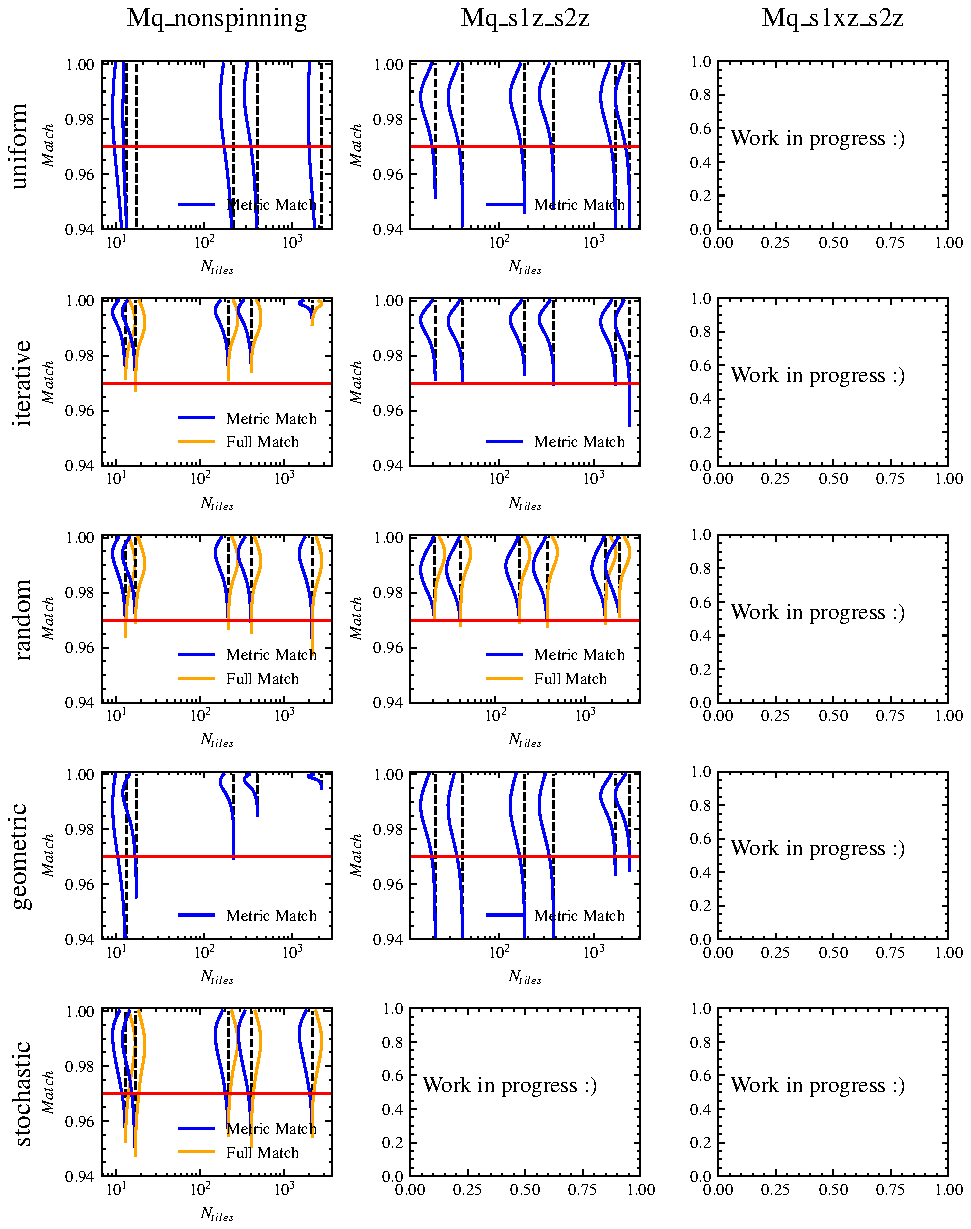
\includegraphics[width=.85\textwidth,keepaspectratio]{placing_validation}
	\caption{Results for the validation of the placing methods on $0.97$ minimum match banks. Each row refers to a different placing method whereas each column refers to a different manifold. In each plot, we report with a cross the number of tiles $N_{\text{tiles}}$ against the number of templates $N_{\text{templates}}$.
	The diamond plot refers to the fitting factor distribution of an injection study performed on the banks. The fitting factor is computed both with the match (orange) and the metric match (blue). The histograms are normalized to arbitrary units and a red tick marks the $0.97$ match threshold. The upper limit of the histograms always corresponds to the match value of $1$ and the support extends until the 1st percentile of the distribution.
	The histograms are built with $1000$ injections for each bank.
	}
	\label{fig:placing_validation}
\end{figure*}

\subsection{Placing methods accuracy} \label{sec:placing_accuracy}

Here we compare the properties of different placing methods - \textit{uniform}, \textit{random} and \textit{stochastic} - and how they perform for different tilings.
The study is helpful to understand their ranges of applicability and possible limitations in their use.

We consider three different manifolds:
\begin{itemize}
	\item \texttt{Mq\_chi} with coordinates $M, q, \chi $ in the rectangle $[20, 50] \mathrm{M_\odot} \times [1,5] \times [-0.99, 0.99]$, in a frequency window $f\in[10, 1024] \text{Hz}$.
	\item \texttt{Mq\_s1xz} with coordinates $M, q, s_{1}, \theta_1$ in the rectangle $[40, 50] \mathrm{M_\odot} \times [1,5] \times [0, 0.99] \times [0,\pi]$, with $f\in[15, 1024] \text{Hz}$.
	\item \texttt{Mq\_s1xz\_s2z\_iota} with coordinates $M, q, s_{1}, \theta_1, s_\text{2z}, \iota$ in the rectangle $[40, 50] \mathrm{M_\odot} \times [1,5] \times [0, 0.99] \times [\pi/4, 3\pi/4] \times [-0.99, 0.99] \times [\pi/4, 3\pi/4]$, with $f\in[15, 1024] \text{Hz}$.
\end{itemize}
For the first manifold we use the approximant \texttt{IMRPhenomD} \cite{Husa:2015iqa,Khan:2015jqa}, while we use \texttt{IMRPhenomXP} \cite{Hannam:2013oca, Khan:2018fmp, Pratten:2020ceb} for the others.

For each manifold, we generate several tilings with a different number of tiles (setting a different value of max-depth with a constant $\epsilon = 0.1$) and we generate a bank with $0.97$ minimum match.
We will {\it not} use a normalizing flow model to interpolate the metric.

We report the histogram of the fitting factors for both the match and the metric match, computed on a set of $1000$ injections.
We stop the stochastic placement algorithm after $N_\text{max} = 200$ iterations with no new templates, while for the random method we employ $2\times 10^6$ livepoints.
The results are shown in Fig.~\ref{fig:placing_validation}.

First of all, we see that the match (orange curve) and its metric approximation (blue curve) are consistent with each other, marking the robustness of the metric approximation Eq.~\eqref{eq:metric_definition}. This will be further confirmed (with some {\it caveats}) in Sec.~\ref{sec:bank_generation}.

According to Eq.~\eqref{eq:N_templates}, the number of templates $N_{\text{templates}}$ given by the {\it uniform} method is a measure of the volume of the space. For this reason, it is interesting to look at how it depends on the number of tiles.
We note that $N_{\text{templates}}$ grows (sometimes mildly) with the number of tiles until a certain upper limit: an increasing number of tiles provides a better estimation of the overall volume of the space, until the estimation converges in the limit of many tiles. 

Depending on the dimensionality of the manifold, the different placing methods have different performance.
In the low dimensional manifolds \texttt{Mq\_chi} ($D=3$) and \texttt{Mq\_s1xz} ($D=4$), the {\it uniform} method has very poor performance and underestimates the number of templates. In the same two manifolds, the {\it stochastic} method performs very well (especially for a large number of tiles) and the {\it random} method gives a satisfying injection recovery, at the price of a large number of templates (3 times larger than those placed by the stochastic method).

The picture changes for the manifold \texttt{Mq\_s1xz\_s2z\_iota} ($D=6$), where the three methods show similar properties. The best performance is achieved by the {\it random} method, once again, at the cost of a large number of templates.
Moreover, since there is no control of the mutual distance between a proposal and the rest of the bank, it is very likely that some regions will be overcovered (i.e. some templates will be too close to each other).
Unlike the other examples, the {\it uniform} has satisfactory coverage properties, even without reaching the accuracy of the {\it stochastic} method.
%Unlike the other examples, the {\it uniform} doesn't perform as the {\it stochastic} method, both in terms of template number and injection recovery.

To understand our result, the key observation is that in high dimensions, the control over the spacing of the templates performed by the {\it stochastic} method is as crucial as in lower dimensions. Hence the {\it stochastic} method only provides moderate improvement (or no improvement at all) over {\it uniform} or {\it random} methods. As discussed before, this is a well-known feature \cite{Messenger:2008ta, Allen:2021yuy, Allen:2022lqr} of high dimensional template banks and it makes the {\it random} (and similarly the {\it uniform}) method very appealing to cover a high dimensional region of the parameter space.
It is also worth noting that the {\it stochastic} method is order of magnitude slower than the other two, making it less competitive for large banks in high dimensional spaces.

As a final remark, we note that the fitting factors computed with the metric match are widely consistent with the un-approximated ones. This shows the robustness of the metric approximation when it comes to template placement.


\begin{figure}[t!]
	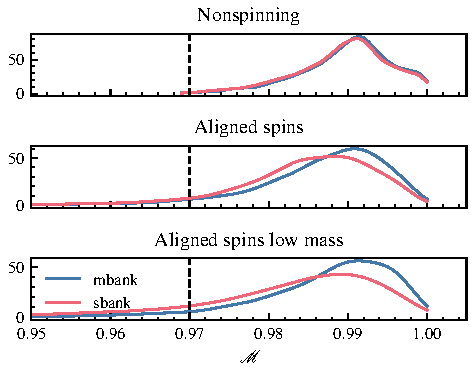
\includegraphics{sbank_comparison}
	\caption{
	Cumulative distribution of the fitting factors of the banks used to compare \texttt{mbank} and \texttt{sbank}. For each parameter space considered, we randomly draw $5000$ points (injections) from the tiling used to generate the \texttt{mbank} bank and we compute the fitting factor of these injections against the two banks. We report the distribution of fitting factor in the histograms. For visualization purposes, we plot the $0.97$ line, which corresponds to the minimum match of the banks.
	The details of the banks generated are reported in Tab.~\ref{tab:sbank_comparison}.
	}
	\label{fig:sbank_comparison}
\end{figure}

\begin{figure}[t!]
	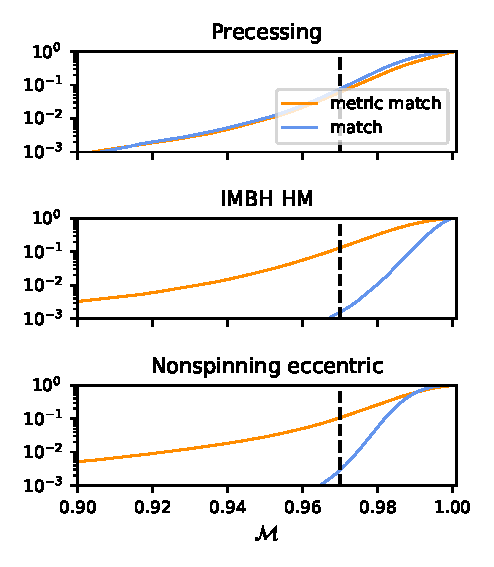
\includegraphics{bank_injections}
	\caption{
	Cumulative distribution of the fitting factors of the three case study banks. Each bank is generated with the normalizing flow interpolation (label ``flow") and without (label ``no flow"). For each bank, we randomly draw $75000$ points (injections) from the tiling and we compute the fitting factor of these injections against the two banks. We report the distribution of fitting factor in the histograms both for the match (both cases) and the metric match (only ``no flow" case). For visualization purposes, we plot the $0.97$ line, which corresponds to the minimum match of the banks.
	The details of the banks generated are reported in Tab.~\ref{tab:casestudy_banks}.
	}
	\label{fig:bank_injections}
\end{figure}


\begin{table*}[t!]
	%\centering
	\setlength\extrarowheight{1pt}
	 \begin{tabular}{l l c c c c} 
	 \toprule
	 	%header
	 \multicolumn{1}{c}{\phantom{Bank name}} & \multicolumn{1}{c}{\textbf{Ranges}} & 
	 \multicolumn{2}{c}{
		\begin{tabular}{c c} \multicolumn{2}{c}{\textbf{Size}}  \\ \texttt{sbank} & \texttt{mbank} \\ \end{tabular}	 
	 } &
	  \multicolumn{2}{c}{
		\begin{tabular}{c c} \multicolumn{2}{c}{\textbf{Time}}  \\ \texttt{sbank} & \texttt{mbank} \\ \end{tabular}	 
	 }\\ 
	 \toprule
	 Nonspinning & \begin{tabular}{@{}l@{}} $M\in [30,50] \mathrm{M_\odot}$ \\ $q\in [1,5]$   \\ \end{tabular}  &
	 		396 & 371 & $O(\text{hours})$ & $O(\text{seconds})$ \\
	\addlinespace[3pt]
	\cdashline{1-6}
	\addlinespace[3pt]
	 Aligned spin & \begin{tabular}{@{}l@{}} $M\in [30,50]$ \\ $q\in [1,5]$ \\ $s_\text{1z}, s_\text{2z}\in [-0.99,0.99]$  \\ \end{tabular}  &
	 	3275 & 4117 & $O(\text{days})$ & $O(\text{minutes})$ \\
	\addlinespace[3pt]
	\cdashline{1-6}
	\addlinespace[3pt]
	 Aligned spin low mass & \begin{tabular}{@{}l@{}} $M\in [10,30]$ \\ $q\in [1,5]$ \\ $s_\text{1z}, s_\text{2z}\in [-0.99,0.99]$  \\ \end{tabular}  &
	 	62009 & 80524 & $O(\text{months})$ &  $O(\text{hours})$\\
	 \bottomrule
	 \end{tabular}
	 \caption{Comparison between the performance of \texttt{mbank} and  \texttt{sbank} on 3 chosen template banks.
	 For each bank, we report the range of parameters covered by the templates, the size of the banks generated by the two methods, as well as the order of magnitude of the generation time. The frequency range for all the banks is $f\in [15,1024] \text{Hz}$.
	 The details of the injection studies are shown in figure~\ref{fig:sbank_comparison}.
	 All the runs have been made on a machine with CPU Intel(R) Xeon(R) CPU E5-2630 installed. Note that the timing numbers for \texttt{sbank} do not account for possible speed up due to parallelization.
	 }
 	 \label{tab:sbank_comparison}
\end{table*}

\subsection{Comparison with \texttt{sbank} }\label{sec:sbank_comparison}

The stochastic template placement code \texttt{sbank} \cite{Ajith:2012mn} is a very common tool used by the LIGO Scientific, Virgo and Kagra Collaborations (LVK) to generate large template banks for analysis and, as such, it has been successfully used in the past three observing runs by several search pipelines for compact binary coalescence \cite{Usman:2015kfa, Mukherjee:2018yra, Aubin:2020goo}. For this reason, it is very important to compare the performance of our code against \texttt{sbank}.
We generate three non-precessing template banks with both \texttt{sbank} and \texttt{mbank}:
\begin{itemize}
	\item A {\it non-spinning} bank
	\item An {\it aligned-spin high-mass} bank
	\item An {\it aligned-spin low-mass} bank
\end{itemize}
The ranges of the parameter space covered by the three banks are reported in Tab.~\ref{tab:sbank_comparison}. All the banks cover the frequency range $f\in [15,1024] \text{Hz}$ and are generated using the PSD measured during the whole second observing run (O2).
For all three banks, \texttt{mbank} templates are placed with the {\it stochastic} method, with $N_\text{max}=300$ and without the use of a normalizing flow model to interpolate the metric. In Tab.~\ref{tab:sbank_comparison} we also report the order of magnitude of the generation time for each bank.
In Fig.~\ref{fig:sbank_comparison}, we report the result of an injection study on the three pairs of banks.

By looking at the banks' size in Tab.~\ref{tab:sbank_comparison}, we observe that \texttt{mbank} consistently places around 30\% more templates than \texttt{sbank}, in the two aligned spins banks. This means that the metric template placement tends to \textit{overcover} the space: it is a known feature (also observed in \cite{Coogan:2022qxs}) and it is inherent to the use of a metric approximation: it is the price to pay for a huge speed-up in the generation.

Looking at the injections fitting factor distributions in Fig.~\ref{fig:sbank_comparison}, we note the fitting factor distribution of \texttt{sbank} and \texttt{mbank} are similar in their shape, even though \texttt{sbank} shows a slightly better performance than \texttt{mbank} in two cases. This suggests that, at least in this simple non-precessing parameter space, \texttt{mbank} is able to match the state-of-the-art performance in covering, in a fraction of the computing time.

%%%%%%%%%%%%%%%%%%%%%%%%%%%%%%%%%%%%%%%%%%%%%%%%%%%%%%%


\begin{table*}[t!]
	\centering
	\setlength\extrarowheight{1pt}
	 \begin{tabular}{l l l c c} 
	 \toprule
	 \multicolumn{1}{c}{\phantom{Bank name}} & \multicolumn{1}{c}{\textbf{Ranges}} & \multicolumn{1}{c}{\textbf{Settings}} &  
	 \multicolumn{2}{c}{
		\begin{tabular}{c c} \multicolumn{2}{c}{\textbf{Size}}  \\ $N_{\text{tiles}}$ & $N_{\text{templates}}$ \\ \end{tabular}	 
	 }\\
	 \toprule
	 Precessing & \begin{tabular}{@{}l@{}} $M\in [25,100] \mathrm{M_\odot}$ \\ $q\in [1,5]$  \\ $s_1\in [0,0.99]$ \\$\theta_1\in [0, \pi]$ \\ $f\in [15,1024] \text{Hz}$ \end{tabular}  &
	 \begin{tabular}{@{}l@{}} IMRPhenomXP \\ $\epsilon = 0.1$ \\ max-depth: 11 \\ $N_\text{max} = 200$ \\ $n_\text{layers} = 6$ \\ $n_\text{hidden} = 8$ \end{tabular}  &
	 131418 & 111564 \\
	\addlinespace[3pt]
	\cdashline{1-5}
	\addlinespace[3pt]
	 IMBH HM & \begin{tabular}{@{}l@{}} $M\in [50, 600] \mathrm{M_\odot}$ \\ $q\in [1,5]$  \\ $\chi \in [0,0.99]$  \\ $\iota \in [0,\pi]$ \\ $f\in [10,1024] \text{Hz}$ \\ \end{tabular}  &
	 	 \begin{tabular}{@{}l@{}} IMRPhenomXPHM \\ $\epsilon = 0.2 $ \\ max-depth: 9 \\ $N_\text{max} = 100$\\ $n_\text{layers} = 6$ \\ $n_\text{hidden} = 8$ \end{tabular}  &
	 	30444 & 125506 \\
	\addlinespace[3pt]
	\cdashline{1-5}
	\addlinespace[3pt]
	 Nonspinning eccentric & \begin{tabular}{@{}l@{}} $M\in [10,75] \mathrm{M_\odot}$ \\ $q\in [1,5]$ \\ $e \in [0,0.3]$ \\ $f\in [15,1024] \text{Hz}$ \\ \end{tabular}  &
	 	 \begin{tabular}{@{}l@{}} EccentricFD \\ $\epsilon = 0.1$ \\ max-depth: 10 \\ $N_\text{max} = 100$\\ $n_\text{layers} = 2$ \\ $n_\text{hidden} = 4$ \end{tabular}  &
	 	11736 & 106357\\
	 \bottomrule
	 \end{tabular}
	 \caption{Summary of three case study banks generate with \texttt{mbank}. For each bank generated, we record the variables being sampled and their ranges. We also report the approximant, the hyperparameters $\epsilon$ and max-depth used for the tiling generation, the $N_\text{max}$ termination threshold for the stochastic placement method as well as the architecture of the normalizing flow used.
	 We also show the size $N_{\text{templates}}$ of the bank and the number of tiles $N_{\text{tiles}}$. Results of an injection study are shown in Fig.~\ref{fig:bank_injections}. The templates distribution of the three banks is reported in Fig.~\ref{fig:bank_scatter}.}
 	 \label{tab:casestudy_banks}
\end{table*}


\begin{figure*}[t]
	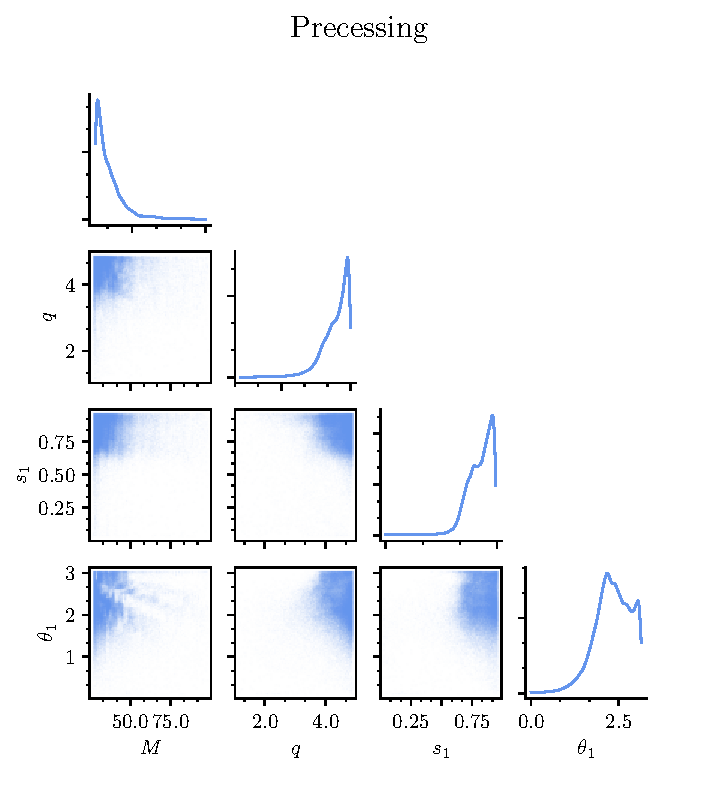
\includegraphics[scale = 0.7]{bank_scatter_Precessing}\hfill
	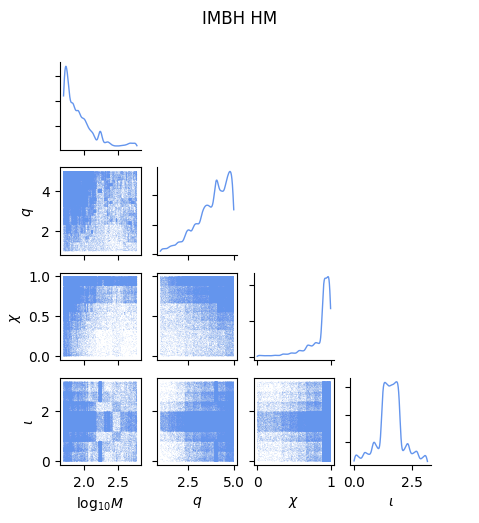
\includegraphics[scale = 0.7]{bank_scatter_IMBH_HM}\hfill
	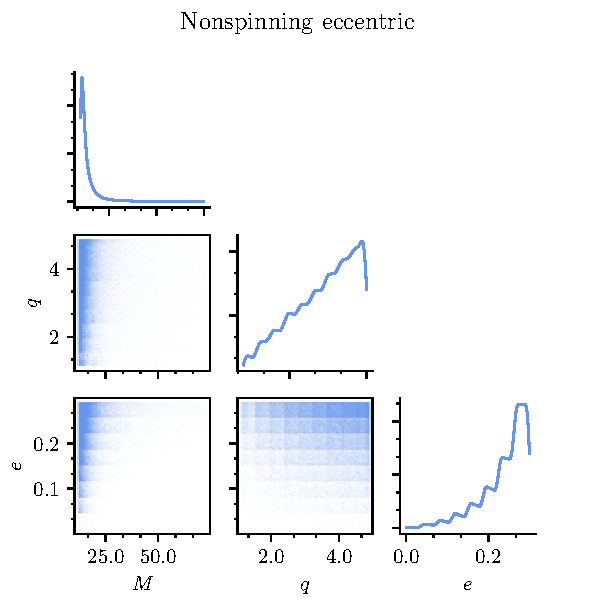
\includegraphics[scale = 0.7]{bank_scatter_Nonspinning_eccentric}
	\caption{Corner plots showing the templates for the three banks described in Tab.~\ref{tab:casestudy_banks}. The masses of each template are parametrized with total mass $M$ and mass ratio $q>1$. In the precessing bank, the spin of the first BH is described by its magnitude $s_1$ and the in-plane angle $\theta_1$. In the HM bank, the templates are described by the effective spin parameter $\chi = s_\text{1z} = s_\text{2z}$ and by the inclination angle $\iota$. In the eccentric bank, besides the masses, we only consider the eccentricity $e$ of the system.}
	\label{fig:bank_scatter}
\end{figure*}

	%%%%%%%%%%%%%%%%%%%%%%%%%%%%%%%%%
\section{Bank generation: three case studies} \label{sec:bank_generation}

To demonstrate the capabilities of our method, we use \texttt{mbank} to generate three large banks, covering interesting regions of the parameter space:
	\begin{itemize}
		\item A precessing BBH bank
		\item An IMBH bank with HMs
		\item A nonspinning BBH eccentric bank
	\end{itemize}
We always use a normalizing flow to interpolate the metric.

For each bank, we perform an injection study with $50000$ injections randomly drawn from the tiling with uniform random sky localization: the results are reported in Fig.~\ref{fig:bank_injections}. We also plot the templates of the banks in Fig.~\ref{fig:bank_scatter}.
In Tab.~\ref{tab:casestudy_banks}, we summarize the features of each bank, such as the size and the range of physical quantities that they cover.
All the banks are generated with a minimum match $MM$ requirement of $0.97$, using the {\it stochastic} placement method.
As above, we use the Hanford detector PSD \cite{O3a_PSDs}.

\subsection{A precessing bank}\label{sec:precessing_bank}
	
In our high-mass {\it precessing} bank, we assign a two dimensional precessing spin to the most massive BH, by considering only the $x$- and $z$-components of the spin $s_1$, sampled in polar coordinates. The masses are sampled in $M,q$-space (total mass, mass ratio)   Thus the metric is evaluated at the coordinates point $\theta = (M, q, s_1, \theta_1)$. We use the approximant \texttt{IMRPhenomXP} \cite{Pratten:2020ceb}.

This choice of variables is based on the fact that the effect of precession can be absorbed in a single {\it effective spin parameter}, assigned to the most massive BH of a binary \cite{PhysRevD.91.024043, PhysRevD.103.083022}. Hence this physical approximation allows us to cover a large number or precessing signals using a (relatively) small number of variables.

By looking at the scatter plots in Fig.~\ref{fig:bank_scatter}, we see the effect due to the discretization error introduced by the tiles: although mitigated by the normalizing flow interpolation, this causes a discontinuity in the template density. Of course, this is unphysical and would be avoided by a non-metric placing method.
Another possible source of discontinuity can be traced back to numerical noise in the numerical gradients of the waveforms. Depending on the approximant, the gradients (hence the metric) may not behave smoothly all across the parameter space, thus explaining (partly) the hard discontinuities.

The injection recovery in Fig.~\ref{fig:bank_injections} is satisfying for both the precessing banks, with around $8\%$ of the $50000$ injections performed having a recovery less than the target match $MM = 0.97$.
The bank coverage can be straightforwardly improved by setting a more stringent termination requirement $N_\text{max}$, which will add more templates with an improvement in injection recovery.

\subsection{An IMBH HM bank}\label{sec:HM_bank}

We generate a bank, covering part of the IMBH region, that includes Higher Order Modes. As HMs are more important in the strong gravity regime, they affect mostly the late inspiral and the merger part of the waveform.
For this reason, it is interesting to search for signals with HM content in the IMBH region, characterized by a total mass $M>50 \mathrm{M_\odot}$. An IMBH signal spends only a small time ($O(ms)$) in the detector's frequency band and thus an accurate HM template is crucial for better detection.
We include in the bank the variables $\left( \log M, q, \chi, \iota \right)$, where $\chi=s_\text{1z}=s_\text{s2z}$ is the effective spin parameter and $\iota$ is the inclination angle.
As before in Tab.~\ref{tab:sbank_comparison}, we report the ranges for each of this quantities. We use the modern HM approximant \texttt{IMRPhenomXPHM} \cite{Pratten:2020ceb}.

The inclusion of HM makes the bank much larger (in other words, the volume of the space is larger). For reference, a non-HM bank, covering the masses and $\chi$ ranges (of course, without $\iota$) has $\sim 1000$ templates. That is 2 orders of magnitude difference!

By looking at the injection recovery in Fig.~\ref{fig:bank_injections}, it is striking to see the discrepancy between the fitting factor computed by the metric and the un-approximated one. Indeed, in the HM case, the metric strongly {\it underestimates} the match, yielding an overpopulated bank. Approximately $15\%$ of the injections have a {\it metric} match recovery below $0.97$: this is consistent with the placing method used, which only ``knows" about metric matches. On the other hand, only $\sim 1\%$ are below $0.98$. The bank generated is effectively a $98\%$ bank.
The cause of such discrepancy is unknown and requires more investigation.

\subsection{An eccentric nonspinning bank}\label{sec:eccentric_bank}

Traditionally, BBH searches have focused on circular orbits.
This is theoretically well-motivated, as by the time of merger, most of the initial orbital eccentricity will be radiated away \cite{Maggiore:2007ulw, Blanchet:2013haa}. Nevertheless it is interesting to search for such signals, since their detection will provide invaluable information on the BBH dynamics as well as the BBH formation channels and stellar evolution.
Eccentricity leaves a characteristic signature on the inspiral; thus it will be more detectable on long signals. For this reason, we focus on the {\it low} mass region $M\in [10,75] \mathrm{M_\odot}$, where the inspiral is detectable for a longer time.
To generate our eccentric bank, we use the approximant \texttt{EccentricFD} \cite{PhysRevD.93.124061} and we limit ourself to low eccentricities $e<0.3$, where the WF modelling is more reliable. Being a Post-Newtonian model, it does not include the merger and the waveform is cut in the late inspiral, as done by the code \texttt{lalsimulation} \cite{lalsuite}. Of course, this removes interesting physics and the resulting bank is expected to have a lower number of templates than what would be obtained by a fully eccentric approximant.
As in the case of the HM bank, the addition of eccentricity delivers a bank orders-of-magnitude larger than a standard non-eccentric bank.

From the scatter plot in Fig.~\ref{fig:bank_scatter}, we note that the discontinuities introduced by the metric are less visible than in the previous cases. This is due to the smaller dimension of the space (3 versus 4 of the previous cases), which makes it easier to tile the space. Moreover, since the approximant \texttt{EccentricFD} is analytic, the metric has a smoother dependence on the parameters, which may also help to avoid discontinuities in template density.

\section{Final remarks and future prospects} \label{sec:conclusion}

We present a novel method to generate template banks covering a high dimensional manifold of (possibly) precessing/HM/eccentric BBH signals.
We rely on the metric approximation to the match in Eq.~\eqref{eq:metric_definition} to compute distances between points and we set up an algorithm to create a tiling of the manifold. Given a tiling, we are able to implement several strategies to place templates, covering the space with a minimum match target.
A normalizing flow model can be optionally used to interpolate the metric, providing more efficient coverage.
Our code is publicly available as a package \texttt{mbank} and it comes with a number of tools to make the bank generation and validation easy.

To validate our method, we compare the output of our code to the the state-of-the-art stochastic placement code \texttt{sbank}. We find that mbank is able to faithfully cover the space, although with a larger number of templates when compared with \texttt{sbank}.
To demonstrate the capabilities of our code, we generated three banks covering some interesting and mostly unexplored regions of the parameter space and we found that \texttt{mbank} is able to provide faithful coverage.
Future work should also demonstrate the validity of \texttt{mbank} in the case of Neutron Star binaries and/or Black Hole Neutron Star binaries.

\texttt{mbank} is orders-of-magnitude faster than the non-metric state-of-the-art bank generation codes.
This makes our code particularly suitable for a large dimensional parameter space and allows the generation of banks which were hitherto unfeasible, due to computational limitations.
This was possible thanks to three innovative features:
\begin{itemize}
	\item The metric is used consistently everywhere throughout the package
	\item The tiling provides a fast and efficient interface to the metric, making tractable hard problems such as volume estimation and manifold sampling.
	\item The normalizing flow model is able to faithfully interpolate the volume element across the parameter space
\end{itemize}

Our work can be improved and extended in several directions:
\begin{itemize}
	\item {\it Improving the metric computation}. The metric accuracy may not be optimal, especially for large coordinate distance $||\Delta\theta||$. While this has not been shown to negatively affect the template placing, it would still be desirable to have a better estimation of the match. Future developments can work in this direction (see App.\ref{app:metric_definition}).
	
	\item {\it Investigate the performance in the HM/eccentric case}. We observed in Sec.~\ref{sec:HM_bank} that the metric placement overcovers the space, due to the fact that the metric underestimates the match. This is puzzling and requires more investigation.
	
	\item {\it Post-process the bank}. Regardless of the placing method, the templates in a bank may not be placed optimally, creating over(under)-dense regions. This is especially true for the {\it random} placing method. It may be beneficial to add a post-processing step to move or remove some templates, which provides a smaller bank with better coverage \cite{Indik:2017vqq}.
\end{itemize}

As a final remark, we emphasize that our work enables the GW community to run searches on novel regions of the BBH signal parameter space. By cutting the bank generation and validation time by orders of magnitude, the computational cost of searching new regions of the parameter space will be dominated by the actual cost of the analysis rather than the cost of prior steps.
This will allow for optimal resource allocation to search for signatures of precession, eccentricity and/or HMs, hopefully leading to new exciting physics discoveries.

	%%%%%%%%%%%%%%%%%%%%%%%%%%%%%%%%% ACKNOWLEDGMENTS
        \begin{acknowledgments}
		S.S., B.G., and S.C. are supported by the research program of the Netherlands Organisation for Scientific Research (NWO).
		The authors are grateful for computational resources provided by the LIGO Laboratory and supported by the National Science Foundation Grants No. PHY-0757058 and No. PHY-0823459. This material is based upon work supported by NSF’s LIGO Laboratory which is a major facility fully funded by the National Science Foundation.
%		We thank Melissa Lopez Portilla, Aaron Zimmerman and Keith Riles for precious comments.
        \end{acknowledgments}

	%%%%%%%%%%%%%%%%%%%%%%%%%%%%%%%%% APPENDIX
%\newpage
\appendix

\section{Details of the metric computation}\label{app:metric}

In this Appendix we report the details of the derivation of the Eq.~\eqref{eq:metric_expression}, as well as the computation of the Hessian $H$ of the overlap Eq.~\eqref{eq:overlap} in terms of the gradients of the waveform $h(\theta)$. 
In what follows, we define $\rescalar{h_1}{h_2}$ and $\imscalar{h_1}{h_2}$ to be respectively the real and imaginary part of $\scalar{h_1}{h_2}$.

We begin by expanding the quantity $\mathcal{M}(\theta+\Delta\theta,\theta )$ for $\Delta\theta$ around $0$. Since the $\mathcal{M}(\theta+\Delta\theta,\theta )$ has a maximum for $\Delta\theta = 0$, the leading term is quadratic in $\Delta\theta$.
We obtain:
\begin{align} \label{eq:metric_derivation}
	&\mathcal{M}(\theta+\Delta\theta,\theta ) = \max_{\Delta t} \mathcal{O}(\theta + \Delta\theta, \theta, \Delta t) \nonumber\\
	& =	\max_{\Delta t} \left\{ 1+ \frac{1}{2}\left[ \partial_{ij}\mathcal{O} \Delta\theta_i \Delta\theta_j + 2  \partial_{it}\mathcal{O} \Delta\theta_i \Delta t + \partial_{tt}\mathcal{O} (\Delta t)^2 \right] \right\}  \nonumber \\
	&= 1 + \frac{1}{2}\left[ \partial_{ij}\mathcal{O} - \frac{\partial_{it}\mathcal{O} \partial_{jt}\mathcal{O}}{\partial_{tt}\mathcal{O}}\right] \Delta\theta_i \Delta\theta_j
\end{align}
where all the derivatives are evaluated at ${\Delta\theta = \Delta t = 0}$ and the explicit time maximization yields
${\Delta t = -\frac{\partial_{it}\mathcal{O} \Delta\theta_i}{\partial_{tt}\mathcal{O}}}$.

From the above Eq.~\eqref{eq:metric_derivation}, we can read the expression for the metric in Eq.~\eqref{eq:metric_expression} recognizing in the derivatives $\partial\partial\mathcal{O}|_{\Delta\theta, \Delta t = 0}$ the components of the Hessian matrix $H$ of the overlap.

We now compute the Hessian of the overlap as a function of the gradients of the {\it normalized} waveforms. For notational convenience, we set $h_+(\theta_1)e^{ift} = s$, we drop any dependence on $\theta_2$ and we understand $\mu = {i, t}$.
We have:
\begin{align}\label{eq:overlap_grads}
	\partial_{\mu} \mathcal{O} &= \frac{1}{\mathcal{O}} \frac{1}{1-\hat{h}^2_{+\times}}
	\left[
	\rescalar{\partial_\mu\hat{s}}{\hat{h}_+}\rescalar{\hat{s}}{\hat{h}_+} 
	+ \rescalar{\partial_\mu\hat{s}}{\hat{h}_\times}\rescalar{\hat{s}}{\hat{h}_\times} \right. \nonumber \\
	&\left. - \rescalar{\partial_\mu\hat{s}}{\hat{h}_+}\rescalar{\hat{s}}{\hat{h}_\times}h_{+\times}
	- \rescalar{\partial_\mu\hat{s}}{\hat{h}_\times}\rescalar{\hat{s}}{\hat{h}_+}h_{+\times}
	\right]
\end{align}
Differentiating another time, after some rearrangements, we get:
\begin{align}
H_{tt} &= - \rescalar{\hat{h}_+}{\hat{h}_+f^2}
			+ \frac{1}{1-\hat{h}^2_{+\times}} \imscalar{\hat{h}_\times}{\hat{h}_+f}^2 \label{eq:H_tt}\\
H_{ti} &= \imscalar{\hat{h}_+}{\partial_i \hat{h}_+f}
			- \frac{1}{1-\hat{h}^2_{+\times}} \rescalar{\hat{h}_\times}{\partial_i\hat{h}_+} \imscalar{\hat{h}_\times}{\hat{h}_+f} \label{eq:H_ti}\\
H_{ij} &= \rescalar{\hat{h}_+}{\partial_i\partial_j\hat{h}_+}
			+ \frac{1}{1-\hat{h}^2_{+\times}} \rescalar{\hat{h}_\times}{\partial_i\hat{h}_+} \rescalar{\hat{h}_\times}{\partial_j\hat{h}_+} \label{eq:H_ij}
\end{align}

To move further, we express a normalized waveform derivatives in terms of the un-normalized ones:
\begin{align*}
	\bullet&\quad \partial_i \scalar{h}{h} = \scalar{\partial_i h}{h}+ \scalar{h}{\partial_i h} = 2 \rescalar{h}{\partial_i h} \\
	\bullet&\quad \partial_i \hat{h} =\frac{1}{\rescalar{h}{h}^{3/2}} \left[ \rescalar{h}{h}\partial_i h -  \rescalar{h}{\partial_i h} h \right]
	\\
	\bullet &\quad \partial_t \hat{h} = i f \hat{h} = i f \frac{h}{\rescalar{h}{h}} \\
	\bullet &\quad \partial_i \partial_j \hat{h} = \frac{1}{\rescalar{h}{h}^{1/2}} \partial_{ij}h 	+3 \frac{1}{\rescalar{h}{h}^{5/2}} \rescalar{h}{\partial_i h}\rescalar{h}{\partial_j h}h \\
	&- \frac{1}{\rescalar{h}{h}^{3/2}} \left[\rescalar{h}{ \partial_{ij} h} h + \rescalar{\partial_i h}{\partial_j h}  h
		+2\rescalar{h}{\partial_{(i} h} \partial_{j)} h \right]
\end{align*}
where $A_{(ij)} = \frac{1}{2}(A_{ij}+A_{ji})$ denotes symmetrization.

Plugging this into the equations~\eqref{eq:H_tt}-\eqref{eq:H_ij}, we get:
\begin{widetext}
\begin{align}
	H_{tt} &= - \frac{1}{h_{++}} \rescalar{h_+}{f^2 {h_+}}
		+ \frac{1}{1-\hat{h}^2_{+\times}} \frac{1}{h_{++}h_{\times\times}} \imscalar{{h_\times}}{f{h_+}}^2 \label{eq:H_tt_grad} \\
	H_{ti} &= - \frac{1}{h_{++}} \rescalar{h_+}{f \partial_i h_+}
		- \frac{1}{1-\hat{h}^2_{+\times}} \frac{1}{h_{++}h_{\times\times}} \imscalar{{h_\times}}{f{h_+}} \rescalar{{h_\times}}{\partial_i h_+}
		+ \frac{\hat{h}_{+\times}}{1-\hat{h}^2_{+\times}} \frac{1}{h^{3/2}_{++}h^{1/2}_{\times\times}}
			\imscalar{{h_\times}}{f{h_+}} \rescalar{{h_+}}{\partial_i h_+} \label{eq:H_ti_grad}\\
	H_{ij} &= - \frac{1}{h_{++}} \rescalar{\partial_i h_+}{\partial_j h_+}
		+ \frac{1}{1-\hat{h}^2_{+\times}} \frac{1}{h^2_{++}} \rescalar{h_+}{\partial_i {h_+}} \rescalar{{h_+}}{\partial_j {h_+}}
		+ \frac{1}{1-\hat{h}^2_{+\times}} \frac{1}{h_{++}h_{\times\times}} \rescalar{h_\times}{\partial_i {h_+}} \rescalar{{h_\times}}{\partial_j {h_+}} \nonumber \\
		& - \frac{2 \hat{h}_{+\times}}{1-\hat{h}^2_{+\times}} \frac{1}{h^{3/2}_{++}h^{1/2}_{\times\times}}
		\rescalar{h_\times}{\partial_{(i} {h_+}} \rescalar{{h_+}}{\partial_{j)} {h_+}} \label{eq:H_ij_grad}
%
%
%
%	\frac{1}{\rescalar{h}{h}^{2}}  \imscalar{h}{\partial_i {h}} \rescalar{{h}}{{h}f} +\rescalar{h}{\partial_i {h}} \imscalar{h}{hf}
%	&- \frac{1}{\rescalar{h}{h}} \imscalar{h}{\partial_i{h} f } \label{eq:H_ti_grad} \\
	%H_{ij} &=  \frac{1}{\rescalar{h}{h}^{2}} \Big\{ \rescalar{h}{\partial_i {h}} \rescalar{{h}}{\partial_j {h}} +\imscalar{h}{\partial_i {h}} \imscalar{h}{\partial_j {h}} \Big\} \nonumber \\
	%&- \frac{1}{\rescalar{h}{h}} \rescalar{\partial_i h}{\partial_j {h}} \label{eq:H_ij_grad} 
\end{align}
\end{widetext}
where we defined $h_{\cdot*} = \rescalar{h_\cdot}{h_*}$.

Such expressions, together with Eq.~\eqref{eq:metric_expression} fully specify the metric computation.
The gradients $\partial_i h$ of the waveform can be computed with any finite difference scheme or analytically for a limited number of waveform surrogate models \cite{PhysRevD.103.043020, Khan:2020fso, Tissino:2022thn}.

The non precessing limit can be recovered by setting $h_\times = i h_+$ and $h_{+\times} = 0$:
\begin{align}
	H_{tt} &= \frac{1}{h_{++}^{2}} \rescalar{{h_+}}{f{h_+}}^2 - \frac{1}{h_{++}} \rescalar{h_+}{f^2 {h_+}} \label{eq:H_tt_grad_NP} \\
	H_{ti} &= \frac{1}{h_{++}^{2}} \imscalar{h_+}{\partial_i {h_+}} \rescalar{{h_+}}{{h_+}f}
		- \frac{1}{h_{++}} \imscalar{h_+}{f \partial_i{h_+}} \label{eq:H_ti_grad_NP} \\
	H_{ij} &=  \frac{1}{h_{++}^{2}} \Big\{ \rescalar{h_+}{\partial_i {h_+}} \rescalar{{h_+}}{\partial_j {h_+}} +\imscalar{h_+}{\partial_i {h_+}} \imscalar{h_+}{\partial_j {h_+}} \Big\} \nonumber \\
	&- \frac{1}{h_{++}} \rescalar{\partial_i h_+}{\partial_j {h_+}} \label{eq:H_ij_grad_NP} 
\end{align}

\newpage

\section{Alternative definitions for the metric}\label{app:metric_definition}

\begin{figure}[t]
	\centering
	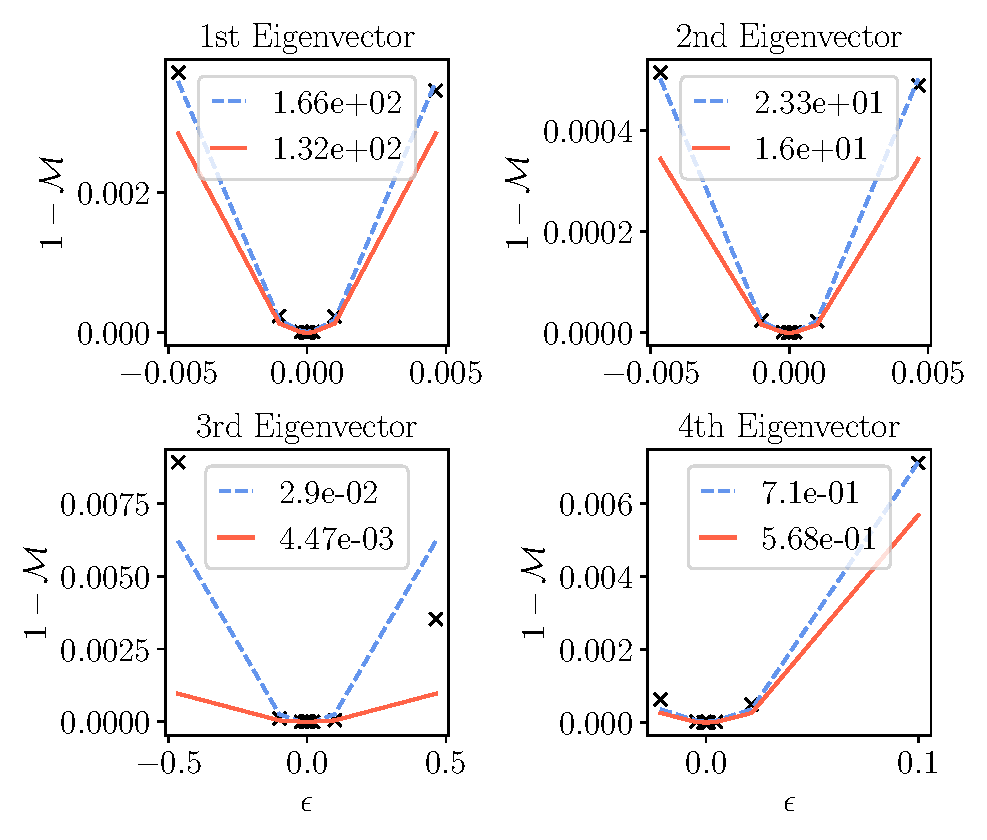
\includegraphics[scale = .55]{parabolae}
	\caption{For each eigenvector of the metric, we compute the empirical relation between the mis-match $1-\mathcal{M}$ and the distance $\epsilon$ of points along the eigenvector direction. The solid line shows the relation predicted by the metric, while the dashed line shows a parabolic fit. In the legend are reported the quadratic coefficients of both lines.}
	\label{fig:parabolae}
\end{figure}

Throughout this paper, we identified the metric with the Hessian of the overlap (see Eq.~\eqref{eq:metric_expression}). While this is widely usd in the literature and has been proven to provide reliable template banks, it still has some non desiderable properties.
To show this, we compute the metric at point $\theta_0 = [20, 3., 0.7, 1.8]$ of manifold \texttt{Mq\_s1xz}, described in Sec.~\ref{sec:placing_accuracy}, and we compute its eigenvalues $\alpha^{(i)}$ and eigenvectors $v^{(i)}$ . We then compute the match $\Mathcal{M}^{(i)}_\epsilon$ between $\theta_0$ and the point $\theta^{(i)}_\epsilon = \theta_0 + \epsilon v^{(i)}$, located at a distance $\epsilon$ along i-th eigenvector.
Finally, we  compute the coefficient $\alpha$ in $1 - \Mathcal{M}^{(i)}_\epsilon = \alpha  \epsilon^2$ by performing a quadratic regression.
In principle, $\alpha$ should be close to the i-th eigenvalue.

In Fig.~\ref{fig:parabolae}, we plot the fitted relation between $1 - \Mathcal{M}$ and $\epsilon$ for each eigenvector, as well as the one computed with the metric. In the legend we report the $a$ coefficient (dashed blue line) and the eigenvalue of the metric (solid orange line).
The striking feature we note in the Figure, is that the eigenvalue is consistently smaller than the fitted $a$ coefficient, sometimes by an order of magnitude.
This means that the hessian, which is computed for $\epsilon\rightarrow 0$, is not able to extrapolate the behaviour of $1 - \Mathcal{M}(\epsilon)$ even at modestly large value of $\epsilon$: the metric approximation to the match loses its predictivity as a measure of distance.
The problem becomes more severe in high dimensional manifolds.
On the other hand, since the banks generated with the hessian metric show nice coverage, one may argue that the {\it volume} estimate provided by the hessian is still accurate enough for our purposes.

As a way out, we could redefine the matrix $M_{ij}(\theta)$, departing from the usual Hessian matrix, to an more suitable expression.
The goodness of the metric expression may depend on the application and on the range of validity of the approximation.
The tensor field $M_{ij}(\theta)$ can be computed through an optimization problem, where we minimize the discrepancy between the two quantities in Eq.~\eqref{eq:metric_definition}, encoded into a {\it loss function}.
The loss function depends on the values of the matrix elements $M^\prime_{ij}$:
\begin{equation} \label{eq:loss_function}
	\mathcal{L}_\theta(M^\prime_{ij}) = \hspace{-4em} \int\limits_{\hspace{3em}\{d(\theta,\theta^\prime) < d_\mathrm{target}\}} \hspace{-3.8em}
		\dvol{\theta^\prime}{D}  \left[ 1 - \mathcal{M}(\theta,\theta^\prime) - M^\prime_{ij} \Delta\theta_i \Delta\theta_j \right]^2
\end{equation}
where the integration extends on a D-ball with radius $d_\mathrm{target}$ centered around $\theta$ and $d_\mathrm{target}$ is a tunable parameter, which controls the validity of the approximation.

At any given point $\theta$, the components $M_{ij}(\theta)$ of the metric are selected by minimizing the above loss:
\begin{equation} \label{eq:metric_optmization}
	M_{ij}(\theta) = \argmin_{M^\prime_{ij}}  \mathcal{L}_\theta(M^\prime_{ij})
\end{equation}
Although the minimization can be tackled with standard techniques, it requires many evaluations of Eq.~\eqref{eq:distance} and sampling from a ``complex" set such as ${\{d(\theta,\theta^\prime) < d_\mathrm{target}\}}$: in most cases this may prove unfeasible.
Future work may try to tackle this optimization problem finding a solution at a feasible computational cost: this may be beneficial to many data analysis applications, such as template placment and Fisher information matrix studies.
A number of alternative metric expression, coming from different heuristic optimization strategies, are already available in \texttt{mbank}, although not fully validated.

	%%%%%%%%%%%%%%%%%%%%%%%%%%%%%%%%% BIBLIOGRAPHY
	\bibliography{biblio.bib}
	\bibliographystyle{ieeetr}

\end{document}



